\section{Планувальники у розподілених обчисленнях}

Планувальники в загальному поділяются на два типи: статичні та динамічні. Статичні мають певне правило розподілу задач на обчислювальні вузли та правило не зміюється під час роботи планувальника. Динамічні планувальники в свою чергу можуть адаптуватися під час роботи та змінювати стратегії планування. Хоч динамічні планувальники і здаються більш універсальними, проте вони дуже складні для аналізу та часто розробляються з метою оптимізації певного параметра.

Основною метою планування є максимізація використання ресурсів та мінімізація часу обробки завдань. Планувальник повинен наказати свої завдання, щоб забезпечити баланс між підвищенням якості послуг і одночасним збереженням ефективності та справедливості серед завдань. Ефективна стратегія планування виконання завдань повинна полягати в тому, щоб досягти меншого часу відгуку, щоб виконання поставлених завдань відбулося в кінцевий строк, як наслідок цього, завдання виконуються, і користувачі можуть надати більше число завдань для хмар підвищення продуктивності хмарної системи.

У програмі "Планування архітектури" користувачі надають свої завдання Центру обробки даних "Брокер", цей брокера веде себе як диспетчер між користувачем та Центром даних і допомагає запланувати завдання на віртуальних машинах. У Центрі даних існує кількість вузлів, на якій кількості віртуальних машин заплановано, і на ці завдання VM заплановано відповідно до політики планування, яку виконує Брокер Центру обробки даних. Номер Data Center Broker схожий на кількість користувачів Cloud. Брокер Центру обробки даних взаємодіє з обласним контролером та запланував подані завдання.

\begin{figure}[H]
	\centering
	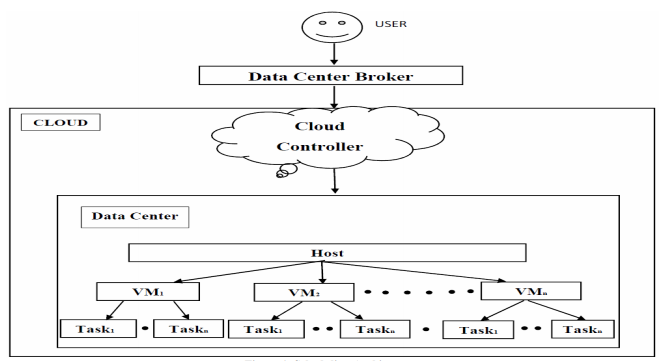
\includegraphics[width=\textwidth]{task_analysis/img/cloud_representation}
	\caption{Ілюстрація структури хмарної обчислювальної мережі}
	\label{fig:cloud_representation}
\end{figure}

Існує дві політики планування: політика спільного планування простору та політики спільного планування часу. У політиці спільного розподілу космічного простору заплановано одне завдання на віртуальну машину в певному екземплярі часу, і після його завершення заплановано ще одне завдання на віртуальній машині. Ця сама політика використовується для планування віртуальних машин на хості. Ця політика поводиться так само, як і алгоритм першого прийому першого сервісу (FCFS).

Кроки політики спільного планування простору:
\begin{itemize}
	\item[Крок 1] Прийняті завдання розташовані в черзі.
	\item[Крок 2] Перше завдання - графік на даній віртуальній машині.
	\item[Крок 3] Це завершує перше завдання, а потім приймаєте наступне завдання з черги
	\item[Крок 4] Якщо черга порожня, вона перевіряє нове завдання.
	\item[Крок 5] Потім повторюється крок 1.
	\item[Крок 6] Кінець
\end{itemize}

У стратегії розподілу часу, що визначає час, вона запланує всі завдання на віртуальній машині одночасно. Він поділив час серед усіх завдань і запланував одночасно на віртуальній машині. Ця політика також використовується для планування віртуальної машини на хості. У цій політиці використовується концепція алгоритму планування круглих ланцюгів (RR).

Кроки політики спільного планування в часі
\begin{itemize}
	\item[Крок 1] Всі прийняті завдання розташовані під чергою.
	\item[Крок 2] Потім заплануйте завдання одночасно на віртуальній машині
	\item[Крок 3] Коли черга порожня, вона перевіряє нові завдання.
	\item[Крок 4] Якщо з'являється нове завдання, то воно заплановано так само, як на кроці 2
	\item[Крок 5] Кінець
\end{itemize}

\begin{figure}[H]
	\centering
	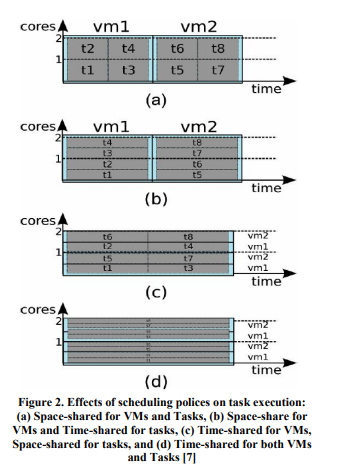
\includegraphics[width=\textwidth]{task_analysis/img/time_space_shared}
	\caption{Ілюстрація планування задач для time та space shared }
	\label{fig:time_space_shared}
\end{figure}

